%\addbibresource{/home/jorgsk/phdproject/bibtex/jorgsk.bib}
\subsubsection{Transcriptome sequencing with RNA-seq}
RNA-seq was introduced in 2008 \cite{nagalakshmi_transcriptional_2008} and has
been used to compare the differential expression of genes, to discover new
genes, and to discover novel isoforms of known genes by finding new
splice-sites and new 5\ppp and 3\ppp terminals \cite{wang_rna-seq:_2009}.

Here we will go through the stages of the RNA-seq experiments that were
performed to produce the data that was analysed as presented in chapter
\ref{chap:polyA}. We will then comment on the stages of the experiment where
biases can be introduced that affect the final result. Finally we will discuss
the matter of mapping the output of RNA-seq -- short RNA sequences called reads
-- to the genome.

\subsubsection{RNA-seq and mapping: the method, errors, and biases}

Here follows a list of steps performed to generate the RNA-seq data that has
been used in this thesis. In the second and forth step, it is necessary to use
poly(T) primes to capture RNA with poly(A) tails. This ensures that poly(A)
tails will be present in the final output.

\begin{enumerate}
	\item The first step for the RNA-seq experiment is to isolate RNA from a
		cell sample obtained from a tissue or a cell culture

	\item Second, the isolated RNA is divided into poly(A)+ and poly(A)-
		fractions. This is done by using a poly(T) primer that binds to the
		poly(A) tail of the mRNA. The RNA that binds the poly(T) primer is
		called the poly(A)+ fraction and the RNA that does not bind the primer
		is separated and called the poly(A)- fraction.

	\item Next, the RNA samples are treated to remove ribosomal RNA. Since
		ribosomal RNA is by far the most abundant species of RNA in the cell,
		its removal will increase the sensitivity for detecting lowly expressed
		transcripts in the sample.

	\item Next, the single stranded RNA is converted into double stranded
        complementary DNA (cDNA). This is required because Illumina sequencers
        sequence DNA and not RNA. To turn RNA into cDNA one anneals primer
        sequences to the RNA template, which are used by the reverse
        transcriptase enzyme for synthesizing cDNA. At this step, it is
        important when studying polyadenylation that at least some of the
        primers are poly(T) primers, otherwise the poly(A) tail itself may not
        be converted into cDNA. Since the poly(T) primers can bind anywhere in
        the poly(A) tail, the lengths of the poly(A) tails in cDNA will be
        reduced compared to those in the original RNA sample. In this step, the
        original single stranded RNA is degraded so only the double stranded
        cDNA remains.

	\item The next step is to fragment the cDNA into smaller pieces, usually by
		sound waves (sonication), to reach a desired average fragment size
		compatible with the sequencing machine (usually around 300 nt),

	\item Finally, short oligonucleotide adapters are added to the 3\ppp and
		5\ppp ends of the cDNA and the cDNA is amplified from these adapters
		with PCR.  PCR amplification is necessary to get the volume of DNA
		required by the sequencing machines. Now the cDNA is ready for
		sequencing.

\end{enumerate}

During sequencing, the double stranded cDNA is split into single strands, and
both strands are sequenced. This has the effect that sequencing outputs the
reverse-transcribed version of the original RNA molecule in addition to the
original. For investigation polyadenylation sites, it is important to note that
this means that usually only the reverse-transcribed leading poly(T) sequence,
and not the poly(A) sequence of the original, will be sequenced (Figure
\ref{fig:polyT_seq}). For example, a polyadenylated 5\ppp CCCGAAAA 3\ppp input
will most often be output as 5\ppp TTTTCGGG 3\ppp from the sequencing machine.
The poly(A) sequence is rarely sequenced because the read length is generally
shorter than the fragment length (76 bp vs 300 bp in Figure
\ref{fig:polyT_seq}), and sequencing happens in the 5\ppp to 3\ppp direction.

It is also important to note that when sequencing homopolymers
(single-nucleotide repeat sequences) like poly(A) or poly(T) stretches, there
is a slight increase in sequencing error rates with the Illumina platform
\cite{minoche_evaluation_2011}. This implies that when sequencing a poly(A)
sequence, other nucleotides than just A may be reported with a higher
probability compared to the rest of the output sequence.

\begin{figure}[htb]
	\begin{center}
		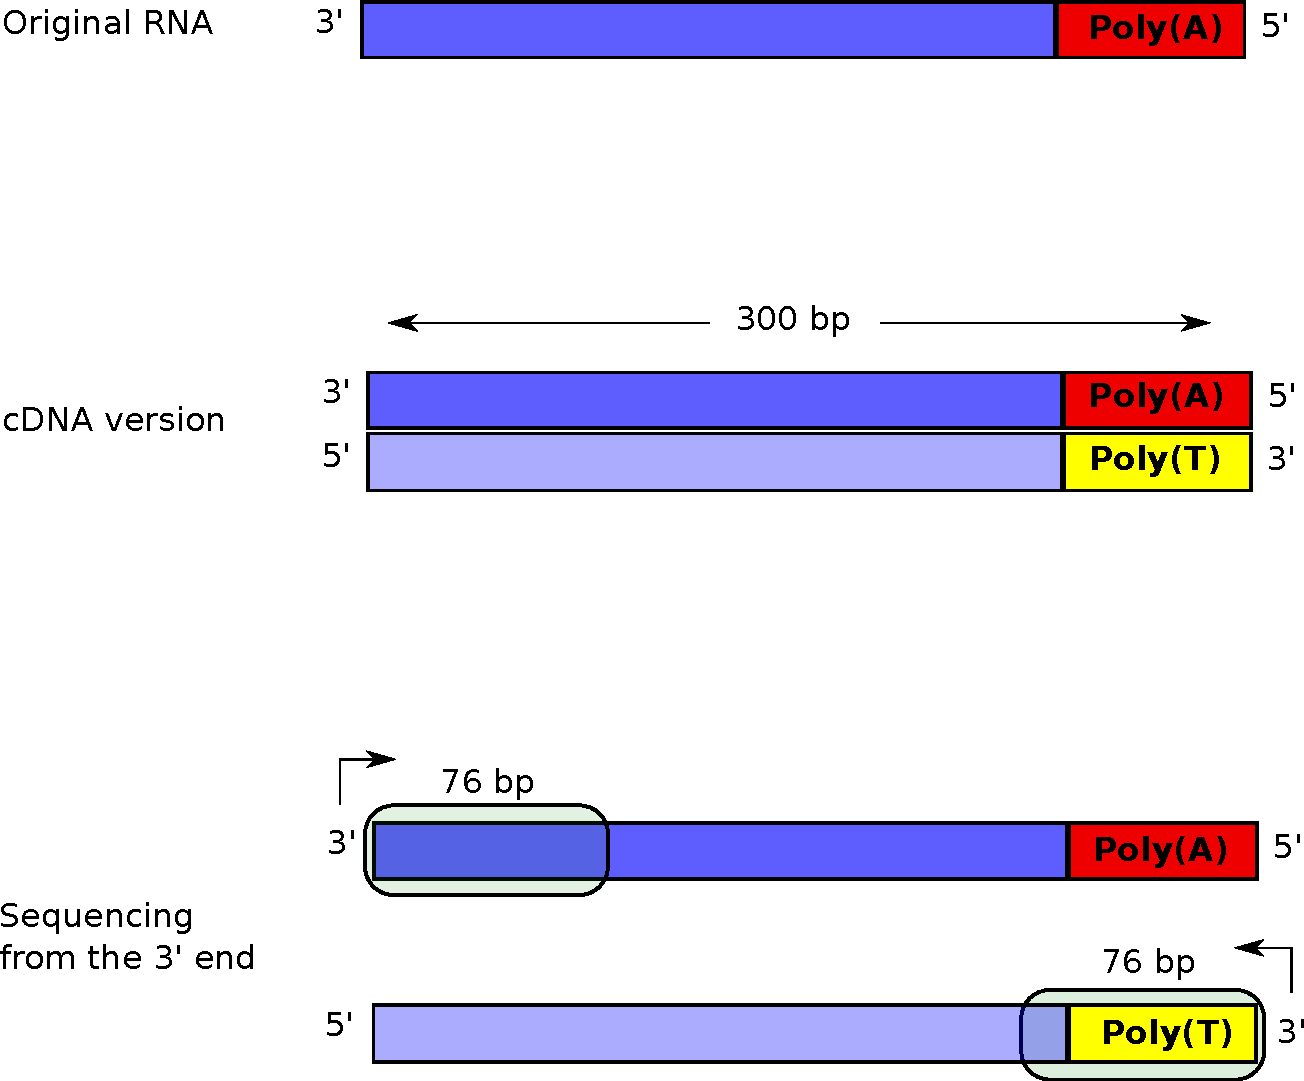
\includegraphics[scale=0.4]{figures/introduction/polyT_sequencing.pdf}
	\end{center}
    \caption{When sequencing polyadenylation sites it is normally the
    reverse-transcribed version of the transcript that is actually sequenced}
	\label{fig:polyT_seq}
\end{figure}

\subsubsection{Mapping reads to the genome}
The sequence-snippets that are output from sequencing machines are called
reads, and generally come in sizes from 30 to 500 basepairs, depending on the
technology used. If a reference genome exists for the organism from which the
RNA sample was taken, these reads can be mapped to that genome by various
pattern-matching algorithms to find out where the RNA originated from
\cite{garber_computational_2011}. All methods used for mapping allow for
mismatches between the read and the genome to allow for errors introduced
through cDNA library creation and sequencing itself.
